\documentclass[11pt]{article}

\usepackage{listings}
\usepackage{graphicx}
\usepackage{tabularx}
\usepackage{subfig}

\begin{document}
\title{Spark-Accelerated Climate Change Analysis}
\author{Jarred Parr}
\date{December 2018}
\maketitle

\section{Introduction}
Climate change is one of the most talked about topics in modern society. From the mainstream media sources, to the President of
the United States, you can't avoid the conversation. This project aims to do some analysis of some of the features of Earth that
would be more directly affected by climate change. The predicted results would primarily be increased wind temperature, and more
severe weather, a product of which being higher wind speeds. This project does analysis on the wind speed variations over the
years and the wind temperature variations. This is in the pursuit of providing a reasonable model to show the affect that climate
change has had in even a short time frame as 3 decades. A linear regressor was used to analyze the data and help determine if,
based on the data, our current trend will likely continue in whatever direction it was found to go, or if it will being to
slowly normalize over time.

\section{Program Architecture}
The software itself is very barebones. The PySpark library takes much of the guesswork out of how to implement things and gives
an easy to use and refreshing interface in which to interact with the underlying structures in place. As a result, the code itself
was extrememly easy to implement and work with. Results were able to be obtained in the use of just two functions which,
realistically, could have been made into just one. There was nothing particularly exemplary discovered in the way of code design
other than that the implementation itself was rather clean and straightforward.

\section{Code}
The code is as follows:

\lstset{frame=tb, language=python}
\begin{lstlisting}
import sys
from collections import defaultdict
from os import listdir
from os.path import isfile, isdir, dirname
from operator import add

from pyspark import SparkContext


def calculate(context, directory, label):
    path_root = '/home/DATA/NOAA_weather/'
    max_speed = defaultdict(int)
    min_speed = defaultdict(int)
    max_temp = defaultdict(int)
    min_temp = defaultdict(int)
    outfile = open('output', 'a+')

    for year in directory:
        lines = context.textFile(path_root + year + '/*')
        speed = lines.map(lambda word: float(word[65:69]) / 10).collect()
        temp = lines.map(lambda word: float(word[87:92]) / 10).collect()
        speed_list = [s for s in speed if s < 300]
        temp_list = [t for t in temp if t <= 300]
        speed_max = max(speed_list)
        speed_min = min(speed_list)
        temp_max = max(temp_list)
        temp_min = min(temp_list)
        temp_avg = sum(temp_list)/float(len(temp_list))

        max_speed[year] = max(speed_max, max_speed[year])
        min_speed[year] = min(speed_min, min_speed[year])
        max_temp[year] = max(temp_max, max_temp[year])
        min_temp[year] = min(temp_min, min_temp[year])

        outfile.write('{} Max Speed: {}\n'.format(year, max_speed[year]))
        outfile.write('{} Min Speed: {}\n'.format(year, min_speed[year]))
        outfile.write('{} Max Temp: {}\n'.format(year, max_temp[year]))
        outfile.write('{} Min Temp: {}\n'.format(year, min_temp[year]))
        outfile.write('{} Average Temp: {}\n'.format(year, temp_avg))


def main():
    if len(sys.argv) != 2:
        print("usage: climate_change data_path", file=sys.stderr)
        sys.exit(1)

    data_path = sys.argv[1]
    dir1980 = []
    dir2000 = []
    for f in listdir(data_path):
        year = None
        try:
            year = int(f)
        except ValueError:
            print('not a number, skipping: {}'.format(f))

        if type(year) is int and year >= 1980 and year <= 1989:
            dir1980.append(f)
        elif type(year) is int and year >= 2000 \
                and year <= 2009 and year != 2004:
            dir2000.append(f)
        else:
            print('out of range, skipping: {}'.format(f))

    sc = SparkContext(appName="CleanCoal")
    calculate(sc, dir1980, '80\'s')
    calculate(sc, dir2000, '2000\'s')
    sc.stop()


main()
\end{lstlisting}
The code relied primarily on batch processing all of the files and performing quick calculations at each index. After discusing
with other colleagues this solution was found to be significantly quicker (>2s) than the options others had attempted to use. This
was found to be because of the just-in-time approach to doing calculation. Performing operations that were dense or branch heavy
inside of the map function took a toll on runtime, python shines when it performs operations on data that needs to be processed,
so instead of bogging down the spark system with potentially dense inference, the python code handles it right before being
compared and indexed.

\section{Results}
Overall the code ran rather quickly. The parallel version took about 20 minutes to run with 24 nodes and the sequential version
was able to complete its task after about 2 hours. which brought a speedup of about 6. The sequential version was run using the
arch lab computers and the distributed version leveraged some arch machines and some of the datacomm machines as well. Overall
the performance was very solid when all things were considered, and python's simple indexing and slicing routines made handling
the data a breeze.


Below are the results and corresponding graphical representation of the ouptut observed.
\begin{figure}[h!]
  \centering
  \subfloat[The Results Table]{{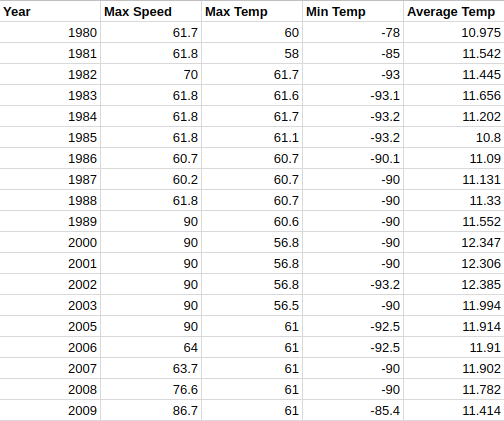
\includegraphics[width=10cm]{table.png}}}%
  \qquad
  \subfloat[The Results Char]{{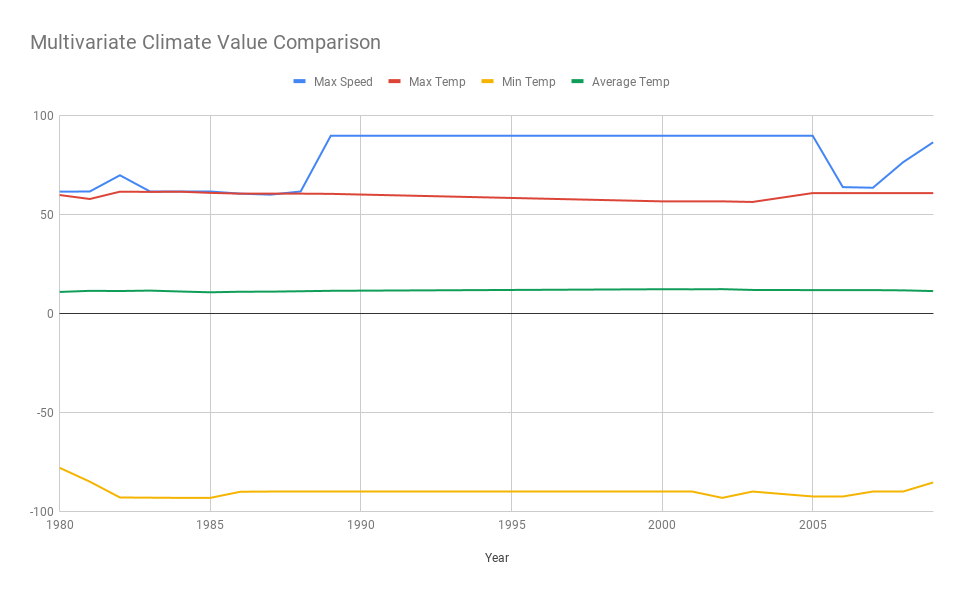
\includegraphics[width=10cm]{chart.png}}}%
  \caption{The visual representation of the output}
\end{figure}
As can be seen, everything is following a very consistent and predictable trend with no major ouliers in any part of the dataset.




\section{Conclusion}
Environmental modeling and prediction is a very important science to not only understand how humans interact with earth, but it
can also give us further inference about the planet's potential to change. This project was exciting and it is very liberating to
know that such a wealth of environmental data exists for study. Using Spark to handle the aggregation of this information was
another useful piece of data aggregation. In my free time I am excited to try and apply it to the context of machine learning
and hope to surmise some sort of realistic model that can make far field predictions about the future of humanity based on current
trends.

\end{document}
